%&pdflatex
\section{Configurazione del software}
Quando Debian avrà finito di installare il sistema di base, nella schermata successiva (Figura \vref{fig:apt-config}) ci verrà chiesto di configurare il \textit{package manager}. Come abbiamo già detto, il package manager è quel programma che serve ad installare le applicazioni. Debian, come package manager, usa \texttt{apt}.

\begin{figure}[ht]
	\centering
	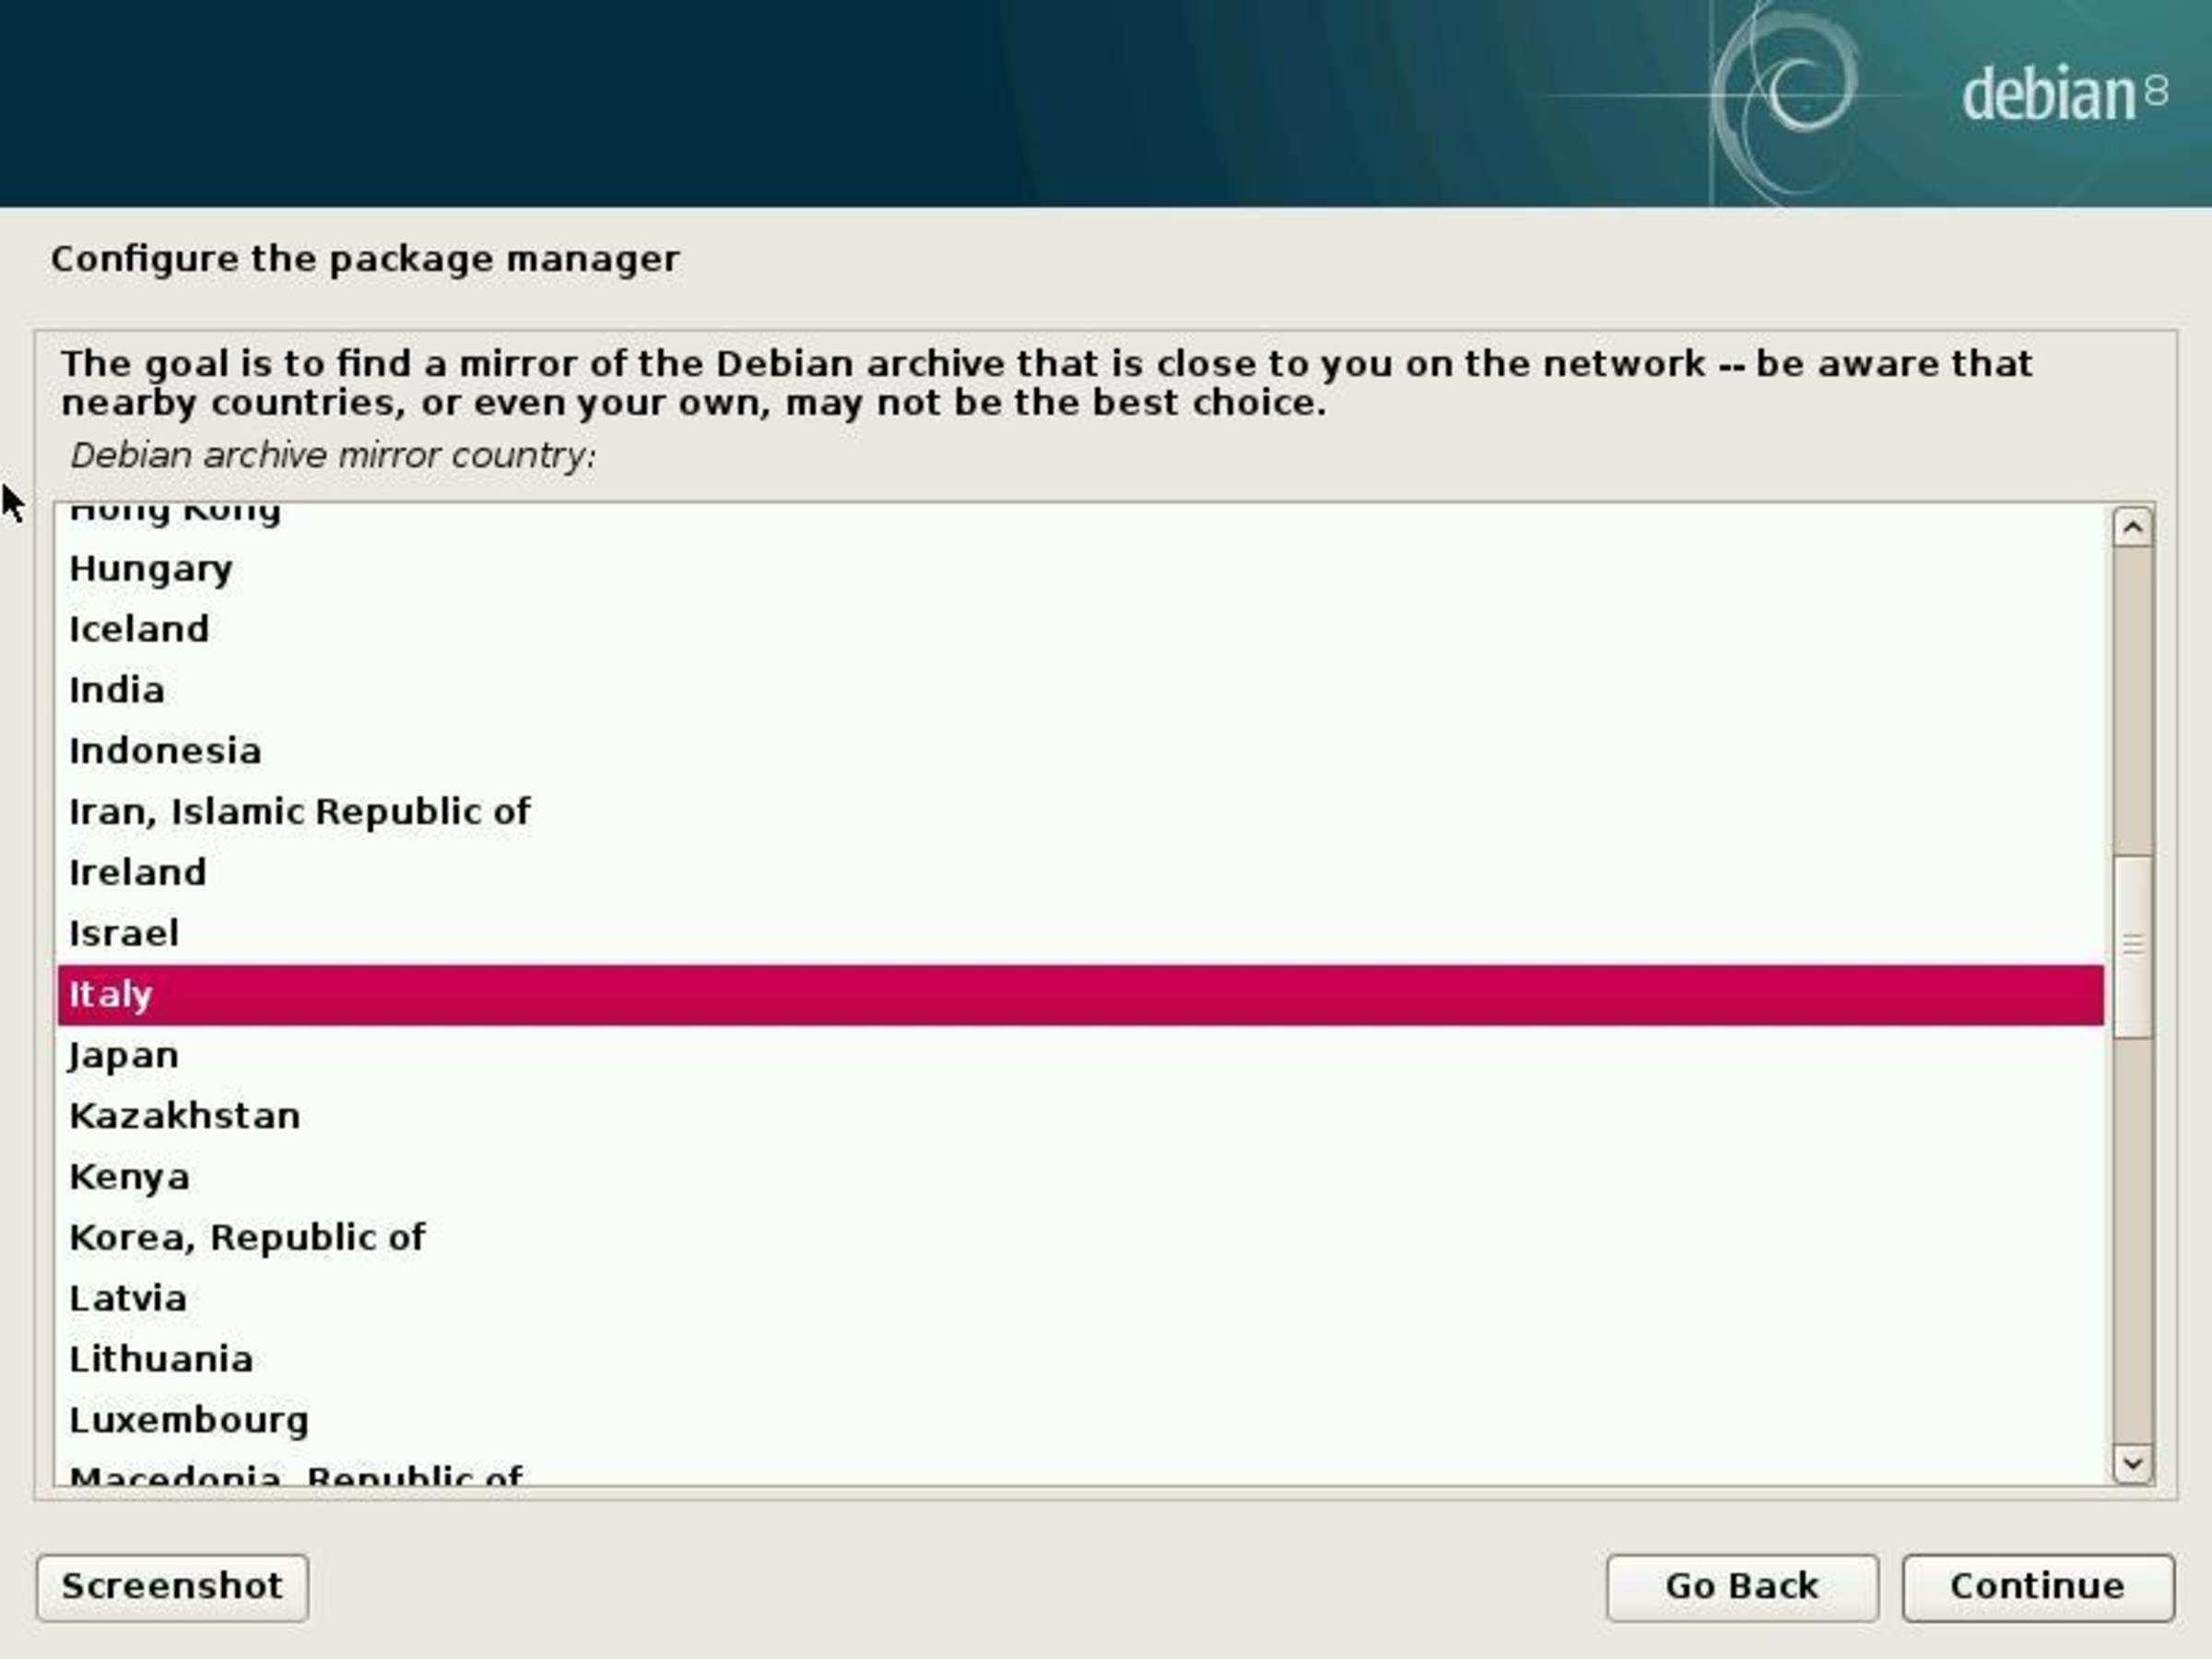
\includegraphics[resolution=600]{apt-config}
	\caption{Configurazione di \texttt{APT}: selezione del paese}
	\label{fig:apt-config}
\end{figure}

Selezioniamo \texttt{Italy} (\texttt{Italia}). Successivamente, ci verrà chiesto di scegliere il \textit{mirror} che si desidera utilizzare per scaricare il software. Tutti i mirror sono uguali, e dovrebbero funzionare ugualmente tutti quanti. Scegliamo \texttt{ftp.it.debian.org}.

Infine, viene chiesto se si desidera utilizzare un \textit{proxy HTTP}. Lasciamo il campo vuoto, ad indicare che non intendiamo utilizzare alcun proxy.

L'installer continuerà adesso ad installare altro software. Dopo un po', ci chiederà se vogliamo partecipare al \textit{popularity contest}, ossia alla raccolta dati anonima per determinare quali sono le applicazioni più utilizzate dagli utenti Debian nel mondo (Figura \vref{fig:popularity-contest}). Il lettore scelga ciò che preferisce.

\begin{figure}[ht]
	\centering
	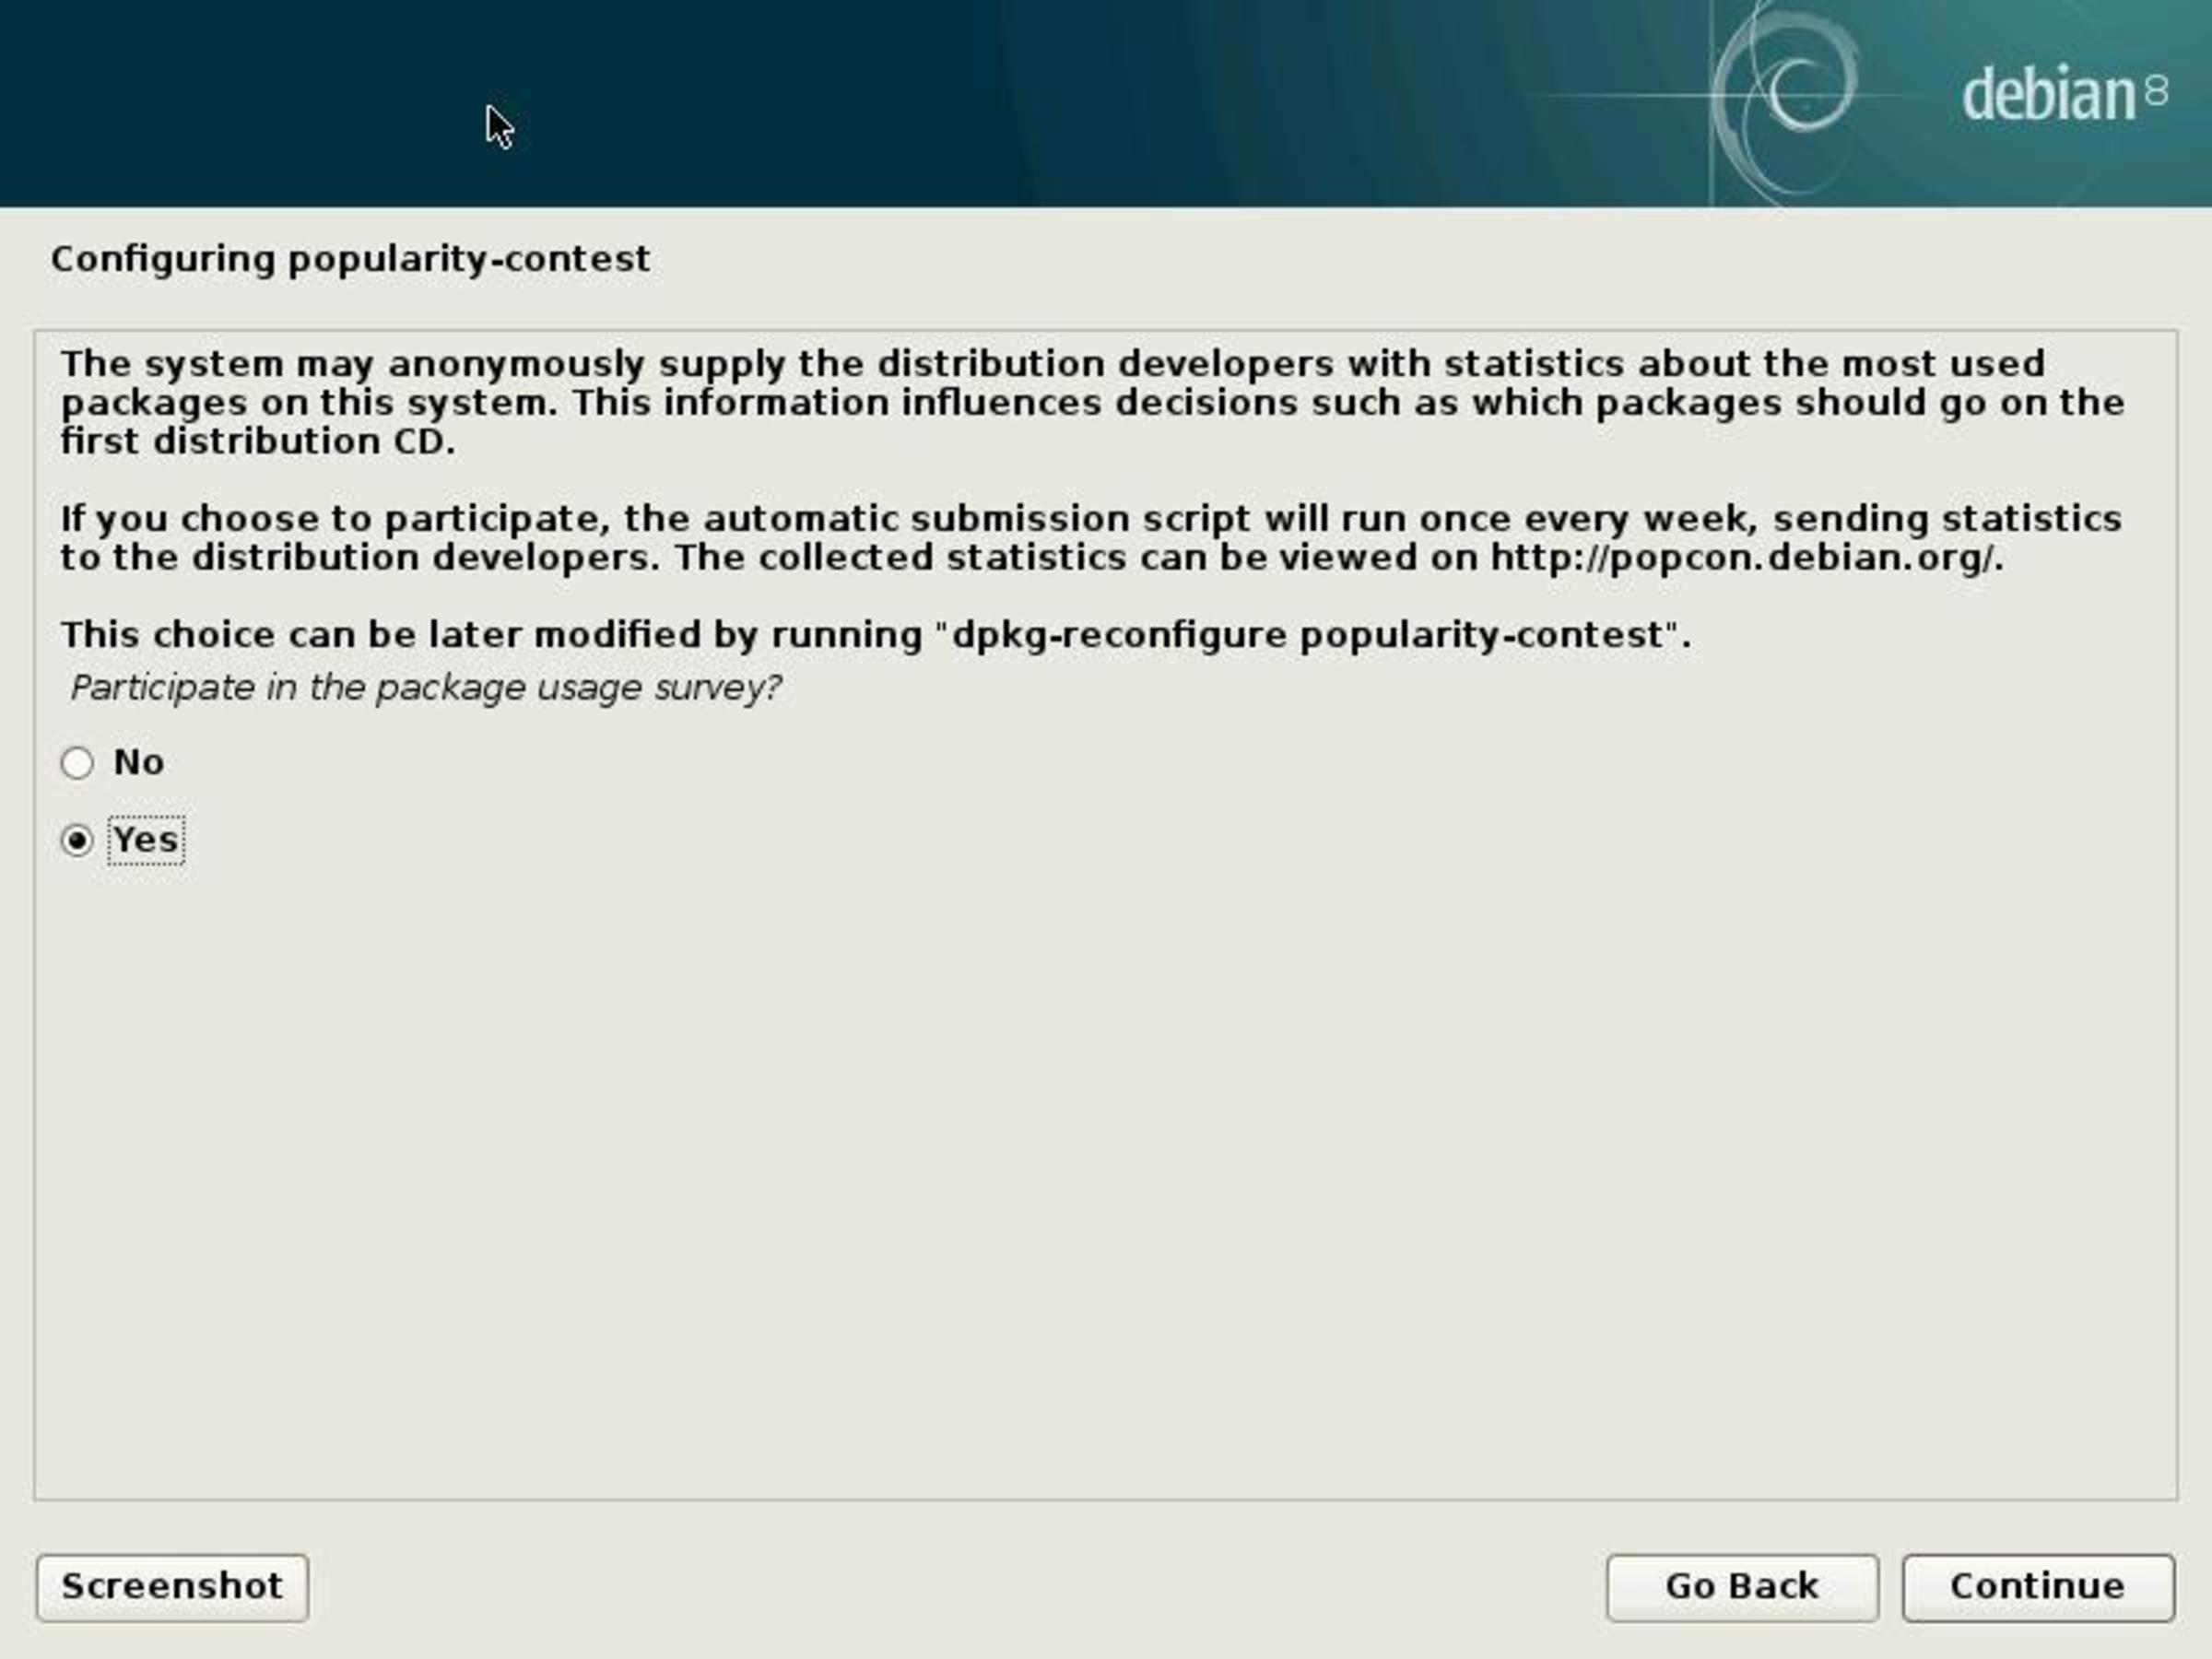
\includegraphics[resolution=600]{popularity-contest}
	\caption{Scelta di partecipazione al \textit{popularity contest}}
	\label{fig:popularity-contest}
\end{figure}

